\documentclass[tikz,border=0pt]{standalone}
\usepackage{iftex}
\ifLuaTeX
\usepackage{fontspec}
\setsansfont{DejaVu Sans}
\else
\usepackage[T1]{fontenc}
\usepackage[utf8]{inputenc}
\usepackage{lmodern}
\fi
\usepackage{amsmath}
\usetikzlibrary{arrows.meta}
\renewcommand{\familydefault}{\rmdefault}
\definecolor{adbg}{HTML}{FFFFFF}
\definecolor{adfg}{HTML}{141414}
\definecolor{admuted}{HTML}{505050}
\definecolor{adline}{HTML}{303030}
\definecolor{adgroup}{HTML}{FAFAFA}
\definecolor{adborder}{HTML}{AAAAAA}
\definecolor{adinput}{HTML}{222222}
\definecolor{adinputfill}{HTML}{FFFFFF}
\definecolor{adcompute}{HTML}{222222}
\definecolor{adcomputefill}{HTML}{FFFFFF}
\definecolor{admodel}{HTML}{222222}
\definecolor{admodelfill}{HTML}{F7F7F7}
\definecolor{admemory}{HTML}{222222}
\definecolor{admemoryfill}{HTML}{F7F7F7}
\definecolor{adtool}{HTML}{222222}
\definecolor{adtoolfill}{HTML}{FFFFFF}
\definecolor{adcontrol}{HTML}{222222}
\definecolor{adcontrolfill}{HTML}{FFFFFF}
\definecolor{adoutput}{HTML}{222222}
\definecolor{adoutputfill}{HTML}{FFFFFF}
\definecolor{adneutral}{HTML}{222222}
\definecolor{adneutralfill}{HTML}{FFFFFF}
\begin{document}
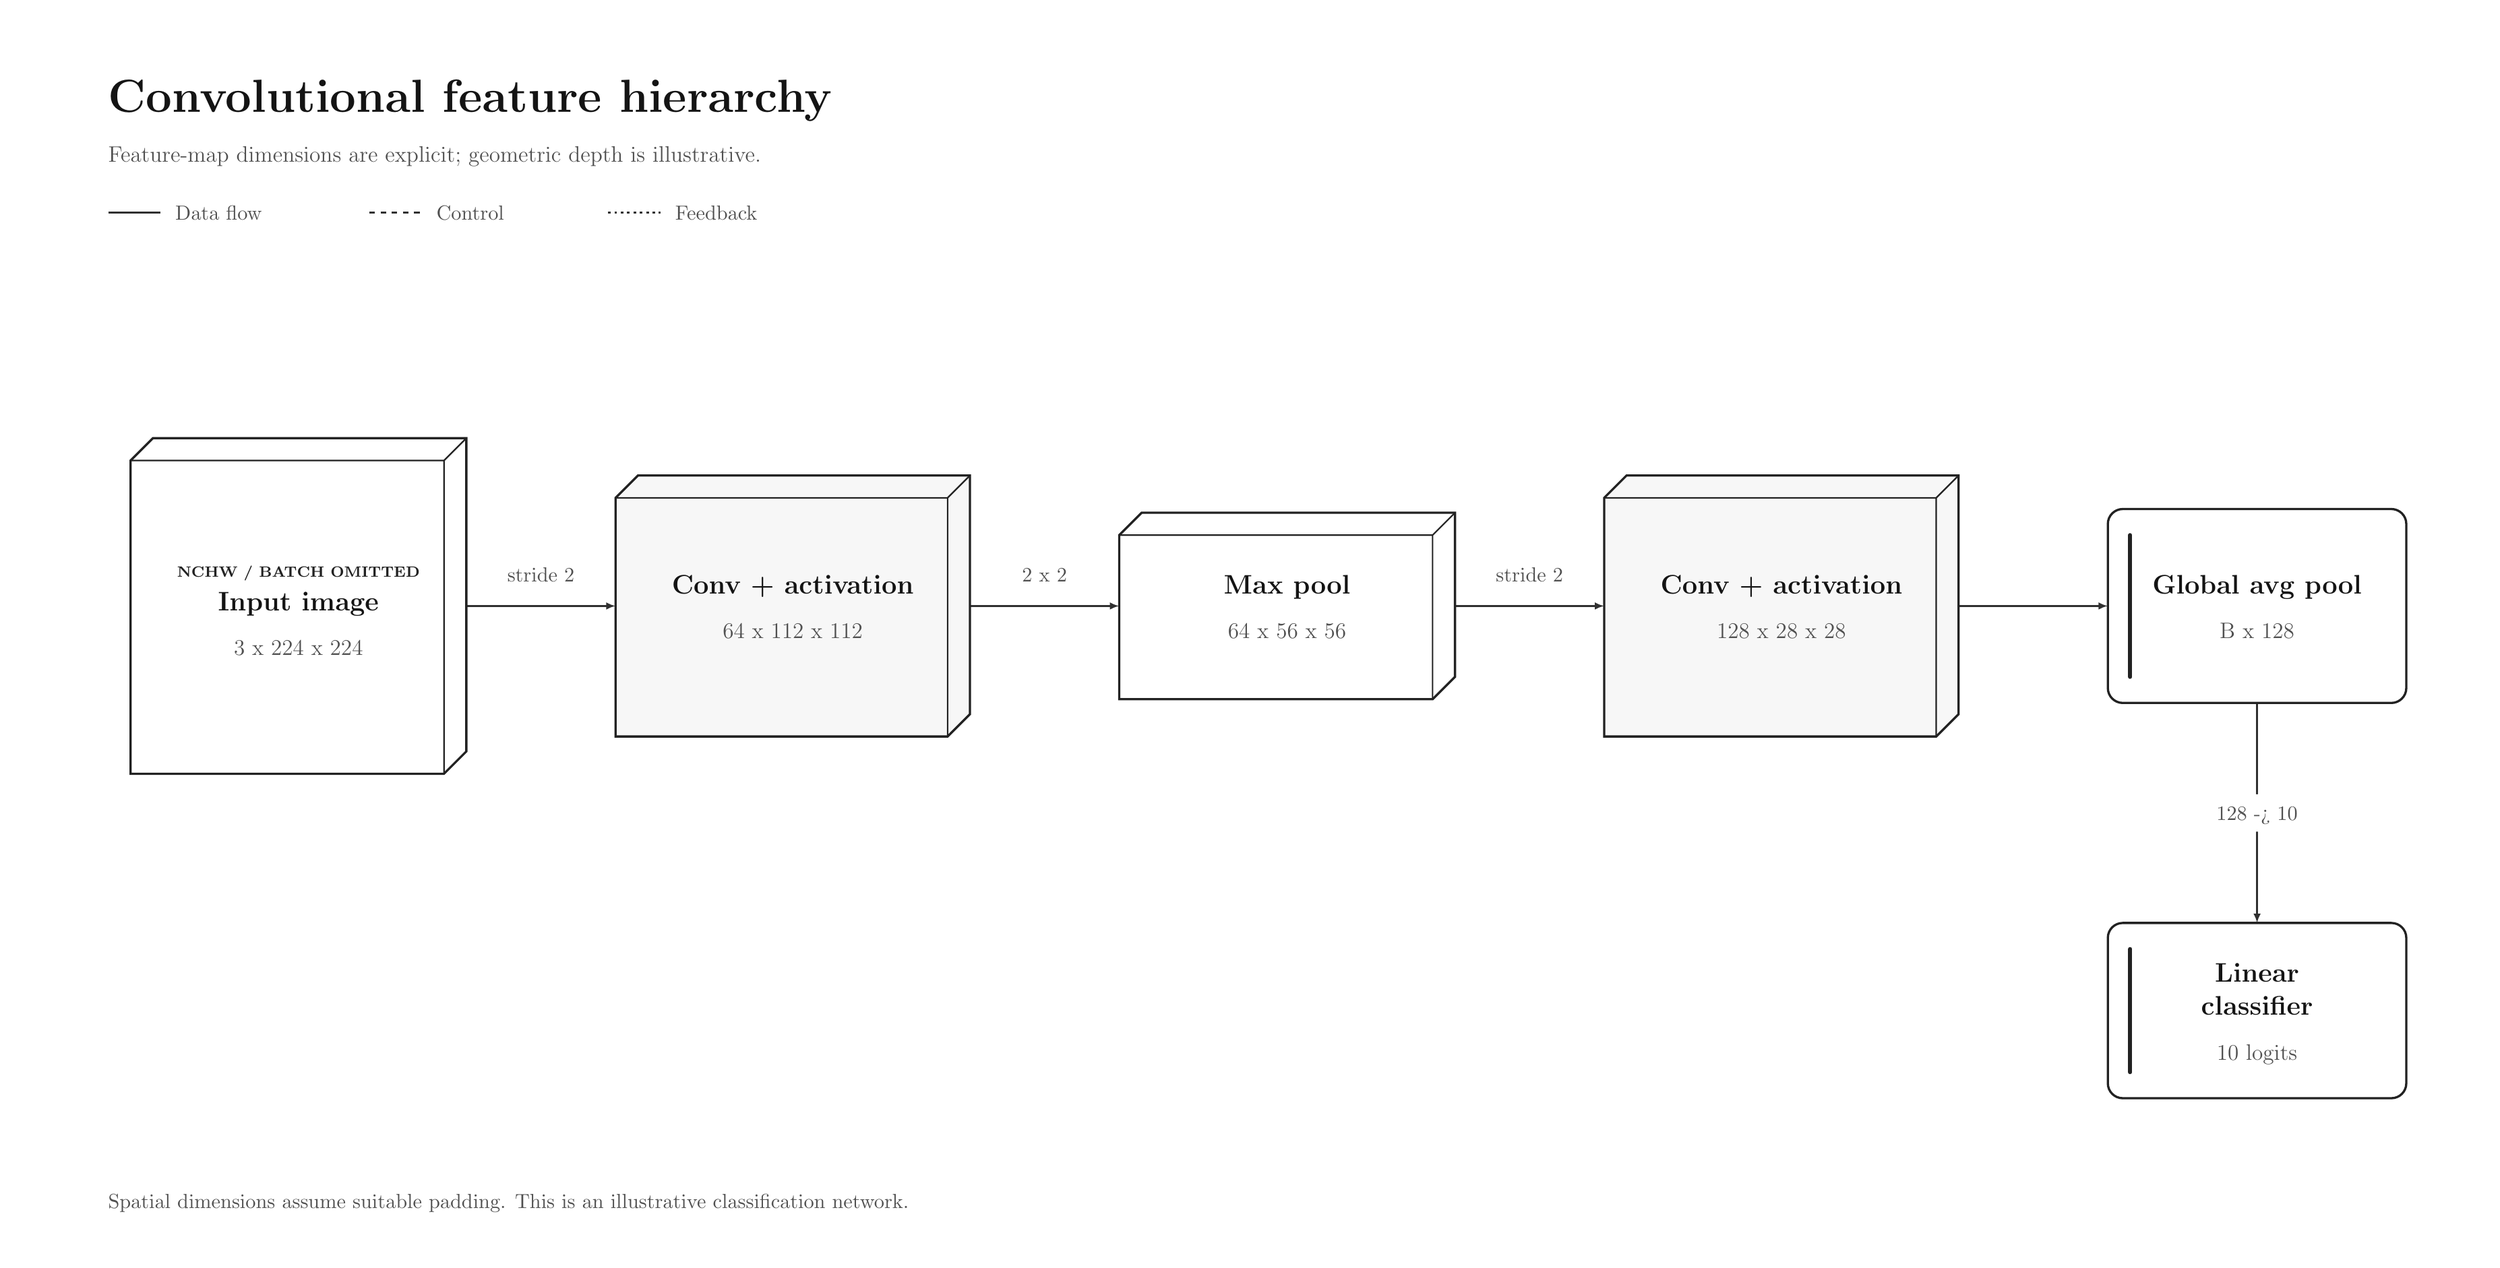
\begin{tikzpicture}[x=1pt,y=-1pt,inner sep=0pt,outer sep=0pt]
\path[use as bounding box] (0,0) rectangle (1320,660);
\fill[adbg] (0,0) rectangle (1320,660);
\node[anchor=base west,text=adfg,font={\rmfamily\fontsize{29}{34.8}\selectfont\bfseries}] at (48,50) {Convolutional feature hierarchy};
\node[anchor=base west,text=admuted,font={\rmfamily\fontsize{13}{15.6}\selectfont}] at (48,77) {Feature-map dimensions are explicit; geometric depth is illustrative.};
\draw[adline,line width=1.4pt] (48,104) -- (76,104);
\node[anchor=base west,text=admuted,font={\rmfamily\fontsize{10.5}{12.6}\selectfont}] at (84,108) {Data flow};
\draw[adline,line width=1.4pt,dashed] (188,104) -- (216,104);
\node[anchor=base west,text=admuted,font={\rmfamily\fontsize{10.5}{12.6}\selectfont}] at (224,108) {Control};
\draw[adline,line width=1.4pt,dotted] (316,104) -- (344,104);
\node[anchor=base west,text=admuted,font={\rmfamily\fontsize{10.5}{12.6}\selectfont}] at (352,108) {Feedback};
\draw[adline,line width=1.3pt,-{Latex[length=5pt,width=4pt]},line join=round] (240,315) -- (280,315) -- (320,315);
\draw[adline,line width=1.3pt,-{Latex[length=5pt,width=4pt]},line join=round] (510,315) -- (550,315) -- (590,315);
\draw[adline,line width=1.3pt,-{Latex[length=5pt,width=4pt]},line join=round] (770,315) -- (810,315) -- (850,315);
\draw[adline,line width=1.3pt,-{Latex[length=5pt,width=4pt]},line join=round] (1040,315) -- (1080,315) -- (1120,315);
\draw[adline,line width=1.3pt,-{Latex[length=5pt,width=4pt]},line join=round] (1200,367) -- (1200,426) -- (1200,485);
\draw[draw=adinput,fill=adinputfill,line width=1.2pt] (60,237) -- (72,225) -- (240,225) -- (240,393) -- (228,405) -- (60,405) -- cycle;
\draw[adinput,line width=0.8pt] (60,237) -- (228,237) -- (228,405) (228,237) -- (240,225);
\node[anchor=base,text=adinput,font={\rmfamily\fontsize{8.5}{10.2}\selectfont\bfseries}] at (150,299.5) {NCHW / BATCH OMITTED};
\node[anchor=base,text=adfg,font={\rmfamily\fontsize{15}{18.0}\selectfont\bfseries}] at (150,317.5) {Input image};
\node[anchor=base,text=admuted,font={\rmfamily\fontsize{11.5}{13.799999999999999}\selectfont}] at (150,341.5) {3 x 224 x 224};
\draw[draw=admodel,fill=admodelfill,line width=1.2pt] (320,257) -- (332,245) -- (510,245) -- (510,373) -- (498,385) -- (320,385) -- cycle;
\draw[admodel,line width=0.8pt] (320,257) -- (498,257) -- (498,385) (498,257) -- (510,245);
\node[anchor=base,text=adfg,font={\rmfamily\fontsize{15}{18.0}\selectfont\bfseries}] at (415,308.5) {Conv + activation};
\node[anchor=base,text=admuted,font={\rmfamily\fontsize{11.5}{13.799999999999999}\selectfont}] at (415,332.5) {64 x 112 x 112};
\draw[draw=adcompute,fill=adcomputefill,line width=1.2pt] (590,277) -- (602,265) -- (770,265) -- (770,353) -- (758,365) -- (590,365) -- cycle;
\draw[adcompute,line width=0.8pt] (590,277) -- (758,277) -- (758,365) (758,277) -- (770,265);
\node[anchor=base,text=adfg,font={\rmfamily\fontsize{15}{18.0}\selectfont\bfseries}] at (680,308.5) {Max pool};
\node[anchor=base,text=admuted,font={\rmfamily\fontsize{11.5}{13.799999999999999}\selectfont}] at (680,332.5) {64 x 56 x 56};
\draw[draw=admodel,fill=admodelfill,line width=1.2pt] (850,257) -- (862,245) -- (1040,245) -- (1040,373) -- (1028,385) -- (850,385) -- cycle;
\draw[admodel,line width=0.8pt] (850,257) -- (1028,257) -- (1028,385) (1028,257) -- (1040,245);
\node[anchor=base,text=adfg,font={\rmfamily\fontsize{15}{18.0}\selectfont\bfseries}] at (945,308.5) {Conv + activation};
\node[anchor=base,text=admuted,font={\rmfamily\fontsize{11.5}{13.799999999999999}\selectfont}] at (945,332.5) {128 x 28 x 28};
\draw[draw=adcompute,fill=adcomputefill,line width=1.2pt,rounded corners=8pt] (1120,263) rectangle (1280,367);
\draw[adcompute,line width=2.2pt,line cap=round] (1132,277) -- (1132,353);
\node[anchor=base,text=adfg,font={\rmfamily\fontsize{15}{18.0}\selectfont\bfseries}] at (1200,308.5) {Global avg pool};
\node[anchor=base,text=admuted,font={\rmfamily\fontsize{11.5}{13.799999999999999}\selectfont}] at (1200,332.5) {B x 128};
\draw[draw=adoutput,fill=adoutputfill,line width=1.2pt,rounded corners=8pt] (1120,485) rectangle (1280,579);
\draw[adoutput,line width=2.2pt,line cap=round] (1132,499) -- (1132,565);
\node[anchor=base,text=adfg,font={\rmfamily\fontsize{15}{18.0}\selectfont\bfseries}] at (1200,516.5) {Linear};
\node[anchor=base,text=adfg,font={\rmfamily\fontsize{15}{18.0}\selectfont\bfseries}] at (1200,534.5) {classifier};
\node[anchor=base,text=admuted,font={\rmfamily\fontsize{11.5}{13.799999999999999}\selectfont}] at (1200,558.5) {10 logits};
\fill[adbg,rounded corners=4pt] (246.8,288) rectangle (313.2,308);
\node[anchor=base,text=admuted,font={\rmfamily\fontsize{11}{13.2}\selectfont}] at (280,302) {stride 2};
\fill[adbg,rounded corners=4pt] (526.25,288) rectangle (573.75,308);
\node[anchor=base,text=admuted,font={\rmfamily\fontsize{11}{13.2}\selectfont}] at (550,302) {2 x 2};
\fill[adbg,rounded corners=4pt] (776.8,288) rectangle (843.2,308);
\node[anchor=base,text=admuted,font={\rmfamily\fontsize{11}{13.2}\selectfont}] at (810,302) {stride 2};
\fill[adbg,rounded corners=4pt] (1163.65,416) rectangle (1236.35,436);
\node[anchor=base,text=admuted,font={\rmfamily\fontsize{11}{13.2}\selectfont}] at (1200,430) {128 -> 10};
\node[anchor=base west,text=admuted,font={\rmfamily\fontsize{11}{13.2}\selectfont}] at (48,638) {Spatial dimensions assume suitable padding. This is an illustrative classification network.};
\end{tikzpicture}
\end{document}
